\apendice{Descripción de adquisición y tratamiento de datos}


\section{Tablas y asociaciones}

Se incluyen a continuación las tablas y asociaciones de los datos llevadas a cabo en este proyecto. 

\subsection{Modelo de Bergman}

Para el Modelo de Bergman, los valores empleados para el estudio de la varaición del umbral de liberación de insulina por el páncreas (parámetro $p_5$) se encuentran en la Tabla \ref{tab:p5}, mientras que aquellos empleados para el estudio de la variación de la tasa de eliminación de la glucosa $p_1$, así como $p_2$ y $p_3$, se incluyen en la Tabla \ref{tab:p123}.

\begin{table}[htbp]
    \centering
    \caption{Valores de $p_5$ comparados.}
    \begin{tabular}{|c|c|c|}
        \hline
          & mg/dL & mmol/L  \\
        \hline
        Caso 1 & 81 & 4.5  \\
        Caso 2 & 85 & 4.722  \\
        Caso 3 & 90 & 5 \\
        Caso 4 & 95 & 5.278 \\
        Caso 5 & 100 & 5.56 \\
        \hline
    \end{tabular}
    \label{tab:p5}
\end{table}

\begin{table}[htbp]
    \centering
    \caption{Valores de p1,p2,p3 empleados en las simulaciones.}
    \begin{tabular}{|c|c|c|c|c|}
        \hline
          & Valor base & Valor aumentado & Valor disminuido \\
        \hline
        p1 & 0.028 & 0.056 & 0.014 \\
        p2 & 0.025 & 0.05 & 0.0125 \\
        p3 & 0.000013 & 0.000026 & 0.0000065 \\
        \hline
    \end{tabular}
    \label{tab:p123}
\end{table}

La simulación correspondiente a la variación de los parámetros p2 y p3 se encuentra en la Sección \ref{sec:variacion_p23} de este anexo.

\subsection{Modelo Modificado}

Respecto a la variación de la constante de tiempo n, los valores empleados para la simulación se disponen en la Tabla \ref{tab:pn}:

\begin{table}[htbp]
    \centering
    \caption{Valores n empleados en la simulación.}
    \begin{tabular}{|c|c|}
        \hline
        Caso & Valor \\
        \hline
        n base & $\frac{5}{54} $\\
        n aumentado (nAum) & $2 \times \frac{5}{54} $\\
        n mitad disminuido (nMitadDis) & $\frac{3}{4} \times \frac{5}{54}$ \\
        n disminuido(nDis) & $\frac{1}{2} \times \frac{5}{54} $\\
        \hline
    \end{tabular}
    \label{tab:pn}
\end{table}

Respecto al ejercicio físico y los planes realizados, se encuentran en las Tablas \ref{tab:ej_previo} y \ref{tab:ej_tras}.

\begin{table}[htbp]
    \centering
    \caption{Casos simulados de ejercicio previo a la ingesta.}
    \begin{tabular}{|c|c|}
        \hline
        Perido previo a la ingesta & Tiempo\\ 
        \hline
        Perido corto & 0 - 60 min \\
        Perido medio & 0 - 120 min \\
        Perido largo & 0 - 180 min \\
        \hline
    \end{tabular}
    \label{tab:ej_previo}
\end{table}

\begin{table}[htbp]
    \centering
    \caption{Casos simulados de ejercicio tras la ingesta.}
    \begin{tabular}{|c|c|}
        \hline
        Perido tras la ingesta & Tiempo\\
        \hline
        Perido corto & 240 - 300 min \\
        Perido medio & 240 - 360 min \\
        Perido largo & 240 - 480 min \\
        \hline
    \end{tabular}
    \label{tab:ej_tras}
\end{table}

Para la combinación de insulinas llevada a cabo unicamente con una finalidad visual para estudiar el efecto en el organismo de su administración, los casos simulados se reúnen en la Tabla \ref{tab:insulinas}.
\clearpage
\begin{table}[htbp]
    \centering
    \caption{Casos simulados en la combinación de insulinas.}
    \begin{tabular}{|c|c|c|}
        \hline
          & Tipo de insulina & Dosis (mg)  \\
        \hline
        Caso 1 & Prolongada & 0.2  \\
        Caso 2 & Rápida, menos dosis & 0.3  \\
        Caso 3 & Rápida, más dosis & 0.6  \\
        Caso 4 & Combinación 1 & Prolongada + Rápida, más dosis \\
        Caso 5 & Combinación 2 & Prolongada + Rápida, menos dosis \\
        \hline
    \end{tabular}
    \label{tab:insulinas}
\end{table}

Para la combinación de la insulina con el ejercicio, se presentan las Tablas \ref{tab:comb_corto} para el periodo de ejercicio corto, y la Tabla \ref{tab:comb_medio} para el periodo medio de ejercicio.

\begin{table}[htbp]
    \centering
    \caption{Casos simulados en la combinación de ejercicio corto e insulina.}
    \begin{tabular}{|c|c|}
        \hline
         & Combinación \\
        \hline
        Caso 1 & Ejercicio periodo corto tras ingesta \\
        Caso 2 & Insulina exógena\\
        Caso 3 & Ejercicio periodo corto + Insulina exógena (1/3 de dosis) \\
        Caso 4 & Ejercicio periodo corto + Insulina exógena (1/2 de dosis) \\
        Caso 3 & Ejercicio periodo corto + Insulina exógena (2/3 de dosis) \\
        \hline
    \end{tabular}
    \label{tab:comb_corto}
\end{table}

\begin{table}[htbp]
    \centering
    \caption{Casos simulados en la combinación de ejercicio medio e insulina.}
    \begin{tabular}{|c|c|}
        \hline
         & Combinación \\
        \hline
        Caso 1 & Ejercicio periodo medio tras ingesta \\
        Caso 2 & Insulina exógena\\
        Caso 3 & Ejercicio periodo medio + Insulina exógena (1/3 de dosis) \\
        Caso 4 & Ejercicio periodo medio + Insulina exógena (1/2 de dosis) \\
        Caso 3 & Ejercicio periodo medio + Insulina exógena (2/3 de dosis) \\
        \hline
    \end{tabular}
    \label{tab:comb_medio}
\end{table}

\subsection{Regulación}


Se incluyen en la Tabla \ref{tab:reg_base} los valores estimados para el regulador obtenido mediante el Método de Prueba y Error, así como los valores del término proporcional empleados para estudiar la variación de este regulador en la Tabla \ref{tab:reg_P}.
\clearpage
\begin{table}[htbp]
    \centering
    \caption{Valores de P y de I estimados mediante el Método de Prueba y Error.}
    \begin{tabular}{|c c|}
        \hline
        Término  & Valor estimado \\
        P & -0.4 \\
        I & 0.00006 \\
        \hline
    \end{tabular}
    \label{tab:reg_base}
\end{table}

\begin{table}[htbp]
    \centering
    \caption{Valores de P empleados para la simulación.}
    \begin{tabular}{|c|c|}
        \hline
        Término Proporcional &  Valor \\
        \hline
        Caso 1 & -0.1 \\
        Caso 2 & -0.4 \\
        Caso 3 & -0.7 \\
        \hline
    \end{tabular}
    \label{tab:reg_P}
\end{table}
Por último, se muestran en la Tabla \ref{tab:val_PI_PID} los valores de Kp, Ti y Td obtenidos para los reguladores PI y PID sintonizados con el Método Basado en Experimentos.

\begin{table}[htbp]
    \centering
    \caption{Valores de Kp, Ti y Td de los reguladores PI y PID empleados para la simulación.}
    \begin{tabular}{|c|c|c|c|}
        \hline
          & $K_p$ &  $T_i$ &  $T_d$ \\
        \hline
        Regulador PI & -0.3195 & 2998.95 &  \\
        Regulador PID &  -0.49 & 2294.06 & 602 \\
        \hline
    \end{tabular}
    \label{tab:val_PI_PID}
\end{table}


\section{Información relevante de las simulaciones}
    
Respecto a los datos obtenidos y la forma de visualizarlos en las simulaciones:
\begin{enumerate}
    \item[-] Todas las simulaciones de la concentración de glucosa en sangre han sido multiiplicadas por un bloque \textit{Gain} con un valor de 18. La finalidad de este producto ha sido la de visualizar las gráficas glucémicas en mg/dL, unidad más popular para la medición de esta variable.
    \item[-] El eje horizontal de las simulaciones correspondiente al tiempo siempre se mide en segundos. El orden de este eje en la mayoría de las simulaciones es de $10 ^4$.
    \item[-] La gran duración de la simulación en la mayoría de los casos se emplea para observar la estabilización de los valores de glucosa e insulina en ellas, así como para mostrar equidad en las simulaciones en cuanto a su duración. En ciertas simulaciones se ha considerado aumentar o disminuir esta duración para observar de mejor manera los resultados.
\end{enumerate}


\subsection{Simulaciones sin resultados concluyentes}

\subsubsection{Variación de los parámetros p2 y p3}
\label{sec:variacion_p23}

Se incluyen a continuación, en las Figuras \ref{fig:p2_gluc} y \ref{fig:p2_ins} las simulaciones correspondientes a la variación del parámetro p2 del Modelo de Bergman.

\begin{figure}[htbp]
    \centering
    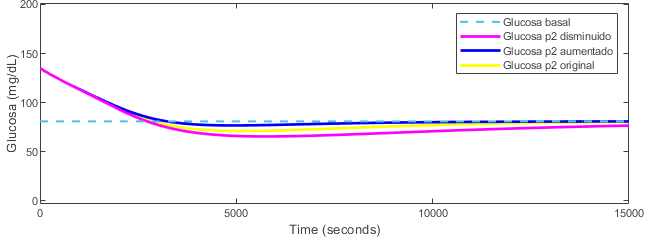
\includegraphics[width=0.9\linewidth]{img/modelo_original/p2_gl.png}
    \caption{Efecto en la glucosa de la variación de p2.}
    \label{fig:p2_gluc}
\end{figure}
\begin{figure}[htbp]
    \centering
    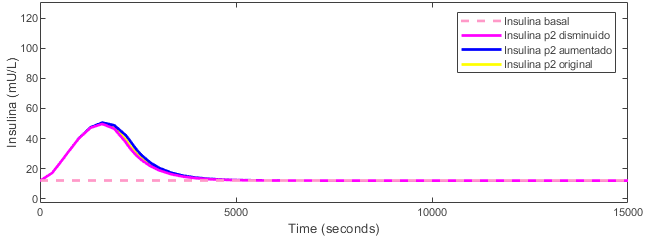
\includegraphics[width=0.9\linewidth]{img/modelo_original/p2_ins.png}
    \caption{Efecto en la insulina de la variación de p2.}
    \label{fig:p2_ins}
\end{figure}
\clearpage
Por último, se muestran en las Figuras \ref{fig:p3_gluc} y \ref{fig:p3_ins} las simulaciones correspondientes a la variación del parámetro p3 en el Modelo de Bergman.

\begin{figure}[htbp]
    \centering
    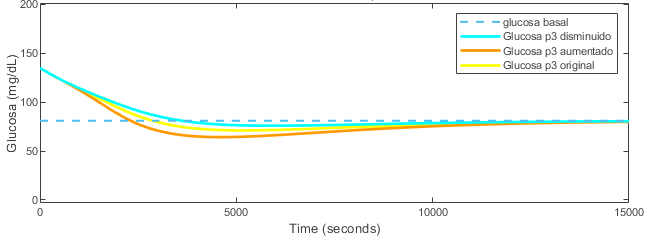
\includegraphics[width=0.9\linewidth]{img/modelo_original/p3_gl.png}
    \caption{Efecto en la glucosa de la variación de p3.}
    \label{fig:p3_gluc}
\end{figure}
\begin{figure}[htbp]
    \centering
    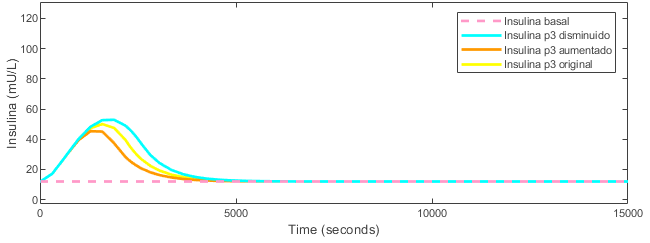
\includegraphics[width=0.9\linewidth]{img/modelo_original/p3_ins.png}
    \caption{Efecto en la insulina de la variación de p3.}
    \label{fig:p3_ins}
\end{figure}

La variación de estos dos parámetros no ha causado diferencias significativas en la glucosa y la insulina del paciente.